\section{Реализация алгоритма решения оптимизационных задач}


\subsection{Задача о замене оборудования}

\indent Перед разработкой программной реализации решения задачи о замене оборудования было приведено аналитическое решение в среде MS Excel и там был автоматизирован процесс нахождения матрицы Беллмана в соответствии с его функциональным уравнением. 

Было принято решение реализовать данный алгоритм на языке программирования Python. По описанной ранее математической модели было реализовано программное обеспечение для решения производственных задач на основе метода динамического программирования. 

Для подсказки сопоставления типов был использован модуль \textit{typing}, а для тестирования был использован модуль \textit{unittest}.
\begin{figure}[h]
  \centering 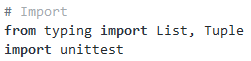
\includegraphics[scale=1]{content/images/impl_equipment1.png}
  \caption{Модули в реализации задачи о замене оборудования.}
  \label{fig:impl_equipment1}
\end{figure}

Была создана функция \textit{replacing\_equipment}, которая решает поставленную задачу. На вход поступает $n$ -- продолжительность работы оборудования (лет), \textit{year} -- возраст оборудования на момент анализа, $s$ -- постоянная остаточная стоимость оборудования, $P$ -- стоимость нового оборудования, $r$ -- список стоимостей продукции, произведённой в течение каждого года планового периода с помощью оборудования,  $u$ -- список ежегодных затрат, связанных с эксплуатацией оборудования.

На выходе функция выводит кортеж, первый элемент которого представляет собой оптимальный план, а второй элемент -- значение целевой функции, то есть максимальная прибыль.
\begin{figure}[h]
  \centering 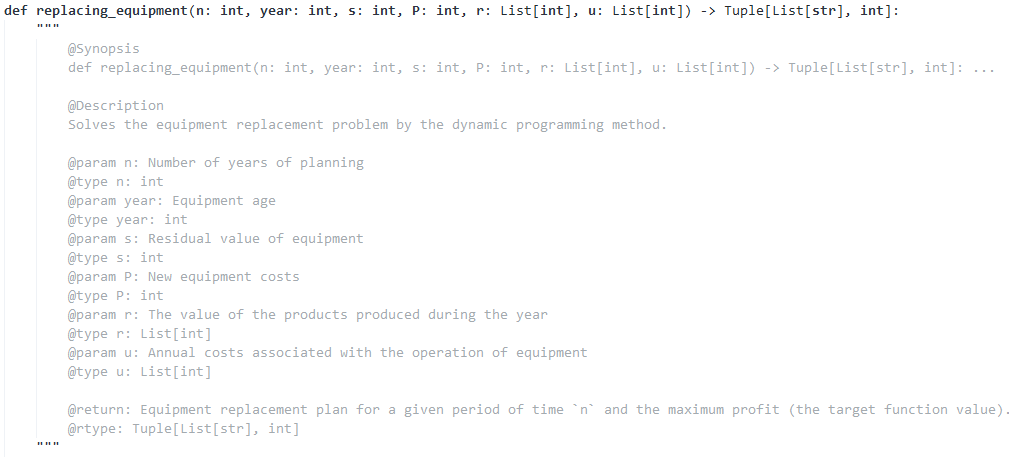
\includegraphics[scale=0.6]{content/images/impl_equipment2.png}
  \caption{Объявление функции.}
  \label{fig:impl_equipment2}
\end{figure}

Далее применяя ранее полученные формулы получаем следующую реализацию условной оптимизации.
\begin{figure}[h]
  \centering 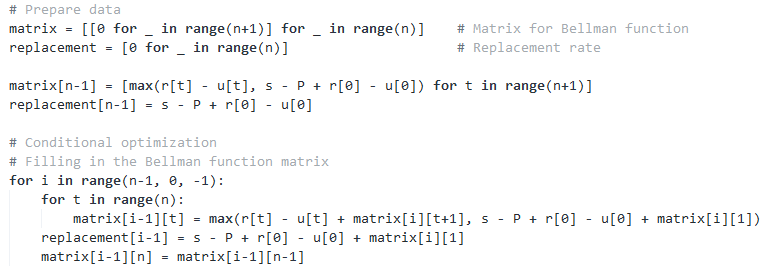
\includegraphics[scale=0.6]{content/images/impl_equipment3.png}
  \caption{Условная оптимизация.}
  \label{fig:impl_equipment3}
\end{figure}

Аналогично поступаем с безусловной оптимизацией.
\begin{figure}[h]
  \centering 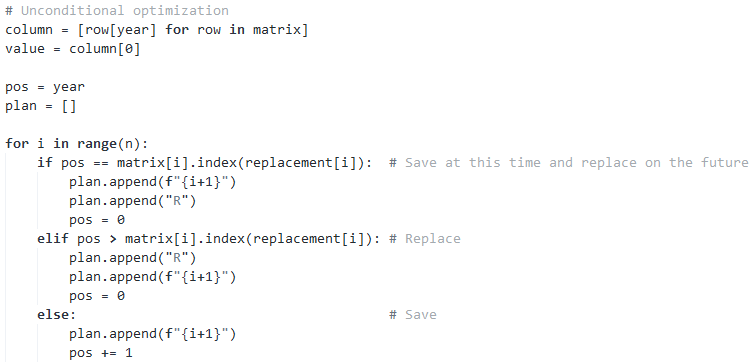
\includegraphics[scale=0.5]{content/images/impl_equipment4.png}
  \caption{Безусловная оптимизация.}
  \label{fig:impl_equipment4}
\end{figure}

Далее были разработаны два теста, для проверки работоспособности программы.
\begin{figure}[h]
  \centering 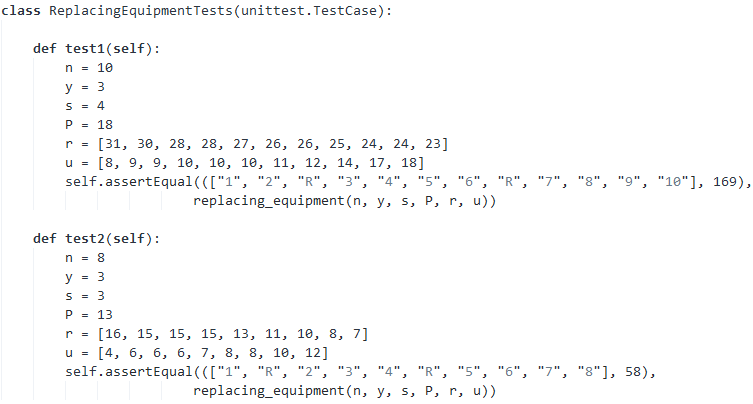
\includegraphics[scale=0.7]{content/images/impl_equipment5.png}
  \caption{Тесты.}
  \label{fig:impl_equipment5}
\end{figure}

Результатом выполнения программы является проверка всех тестов и вывод сообщения об успешном или провальном прохождении этих тестов. 

Полный кода листинг программы указан в приложении. (\hyperref[sec:appendix1]{Приложение А})


\subsection{Задача о рюкзаке}

\indent Перед разработкой программной реализации решения задачи о замене оборудования было приведено аналитическое решение в среде MS Excel и там был автоматизирован процесс нахождения матрицы Беллмана в соответствии с его функциональным уравнением.

Сперва рассмотрим решение, которое было получено в среде MS Excel с помощью надстройки <<Поиск решения>>.

Имеется следующий набор исходных данных.
\begin{figure}[h]
  \centering 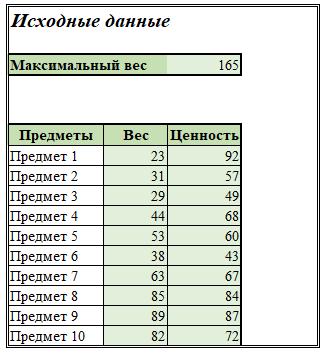
\includegraphics[scale=0.7]{content/images/impl_knapsack1.png}
  \caption{Исходные данные.}
  \label{fig:impl_knapsack1}
\end{figure}

Для решения данной задачи построим вспомогательную таблицу.
\begin{figure}[h]
  \centering 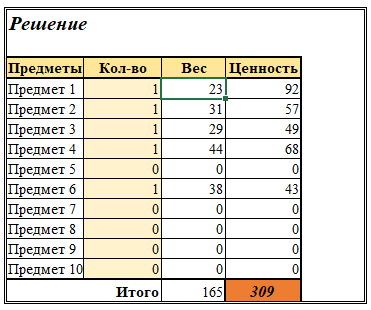
\includegraphics[scale=0.8]{content/images/impl_knapsack2.png}
  \caption{Таблица решения.}
  \label{fig:impl_knapsack2}
\end{figure}

Столбец <<Кол-во>> является столбцом, в котором будут содержаться изменяемые переменные. Столбец <<Вес>> является произведением соответствующей ему количеству, на значения веса предмета в исходных данных, <<Ценность>> будет определяться аналогично. В нижних ячейках указана суммарная ценность, которая будет являться целевой функцией и суммарный вес, который будет являться ограничением.

Исходя из этого мы можем применить <<Поиск решения>>.
\begin{figure}[h]
  \centering 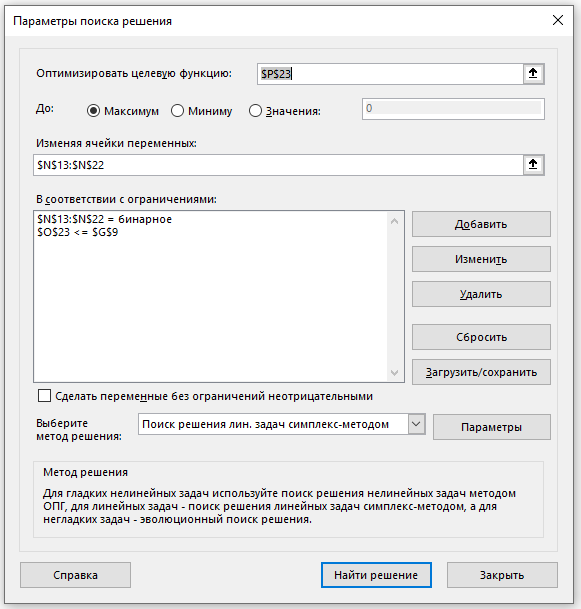
\includegraphics[scale=0.6]{content/images/impl_knapsack3.png}
  \caption{Окно <<Поиск решения>>.}
  \label{fig:impl_knapsack3}
\end{figure}


После этого можно увидеть получившееся решение и определить какие предметы будут входить в итоговый рюкзак, а какие нет.

Также данная задача была решена на языке программирования Rust, в соответствии с теми формулами, которые были рассмотрены при аналитическом решении задачи.

Для определения максимума между числами была использована функция из стандартной библиотеки \textit{max} из модуля \textit{cmp}.
\begin{figure}[h]
  \centering 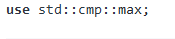
\includegraphics[scale=1]{content/images/impl_knapsack4.png}
  \caption{Модули в реализации задачи о рюкзаке.}
  \label{fig:impl_knapsack4}
\end{figure}

Далее в соответствии с формулами условной оптимизации была создана функция \textit{knapsack\_table}, которая принимает на вход: $w$ -- вес рюкзака, \textit{weights} -- набор весов соответствующих предметов, \textit{values} -- набор стоимостей предметов. На выходе функция возвращает матрицу функции Беллмана.
\begin{figure}[h]
  \centering 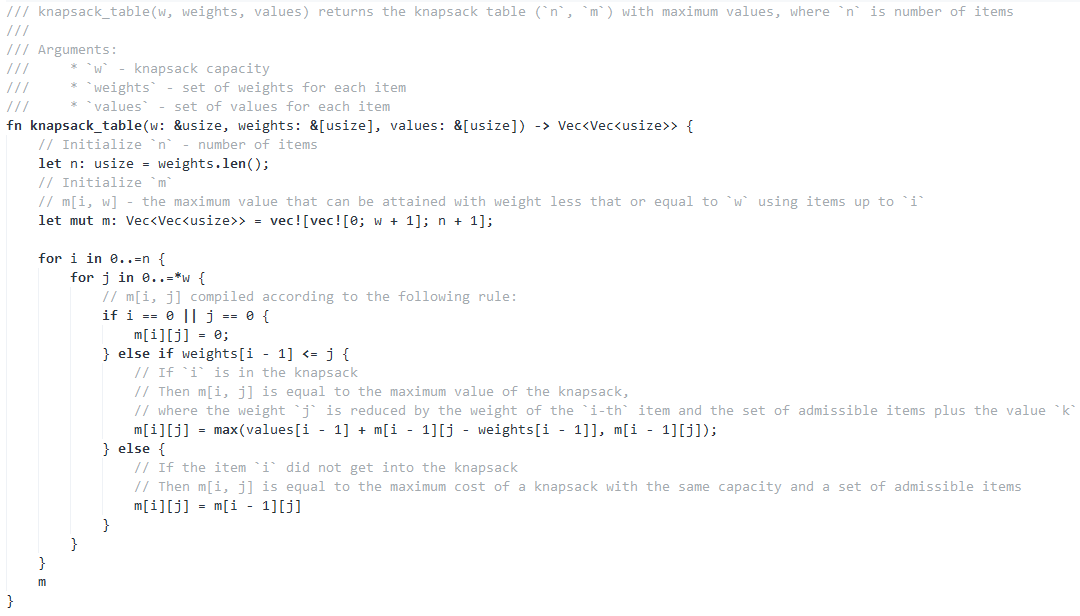
\includegraphics[scale=0.6]{content/images/impl_knapsack5.png}
  \caption{Функция \textit{knapsack\_table}.}
  \label{fig:impl_knapsack5}
\end{figure}

Далее в соответствии с формулами безусловной оптимизации была создана функция \textit{knapsack\_items}, которая принимает на вход: \textit{weights} -- набор весов соответствующих предметов, $m$ -- матрица функции Беллмана, $i$ -- рассматриваемые предметы (для начального значения $i=N$), $j$ -- стоимость рюкзака на соответствующем этапе (для начального значения $j=W$). На выходе функция возвращает список элементов, которые вошли в итоговый рюкзак.
\begin{figure}[h]
  \centering 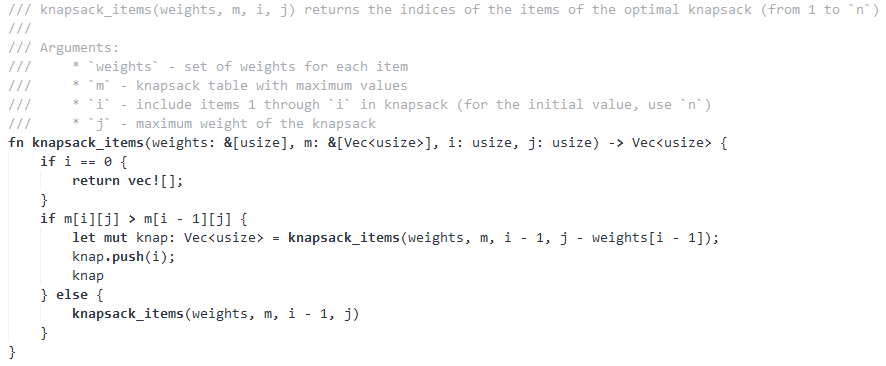
\includegraphics[scale=0.6]{content/images/impl_knapsack6.png}
  \caption{Функция \textit{knapsack\_items}.}
  \label{fig:impl_knapsack6}
\end{figure}

Также была разработана функция \textit{knapsack}, которая объединяет условную и безусловную оптимизацию. Данная функция возвращает кортеж из трёх элементов: первый элемент -- стоимость рюкзака, второй элемент -- вес рюкзака, третий элемент -- набор предметов, вошедших в рюкзак.
\begin{figure}[h]
  \centering 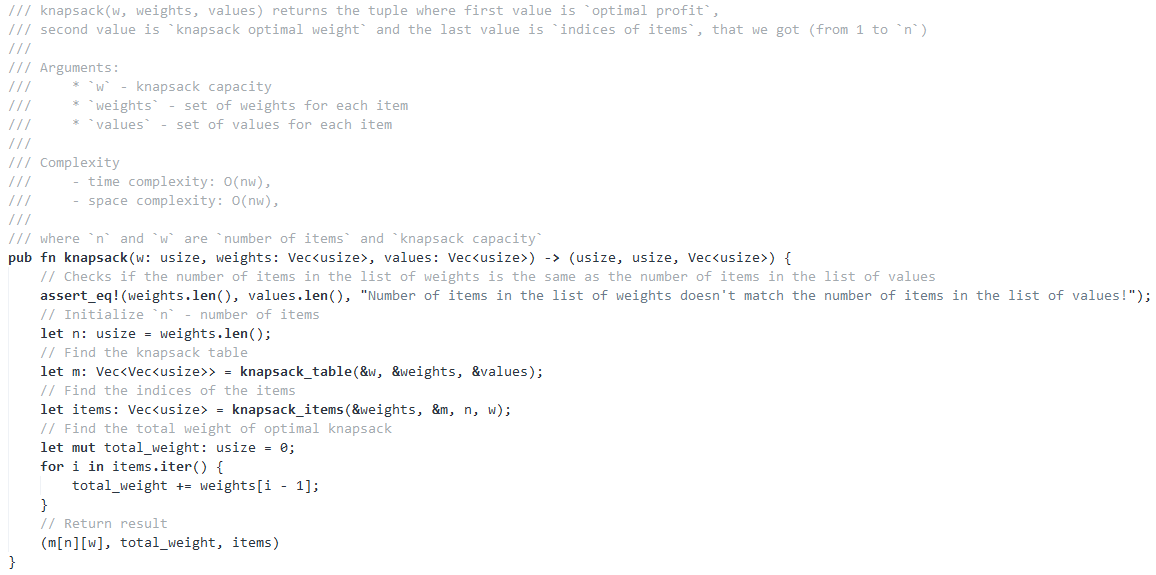
\includegraphics[scale=0.6]{content/images/impl_knapsack7.png}
  \caption{Функция \textit{knapsack}.}
  \label{fig:impl_knapsack7}
\end{figure}

Далее были взяты тесты с бенчмарка, для проверки работоспособности программы.
\begin{figure}[h]
  \centering 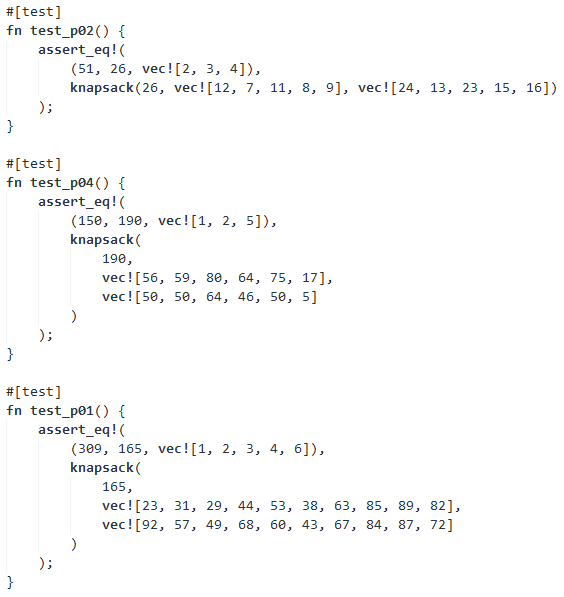
\includegraphics[scale=0.6]{content/images/impl_knapsack8.png}
  \caption{Первый набор тестов.}
  \label{fig:impl_knapsack8}
\end{figure}

\begin{figure}[h]
  \centering 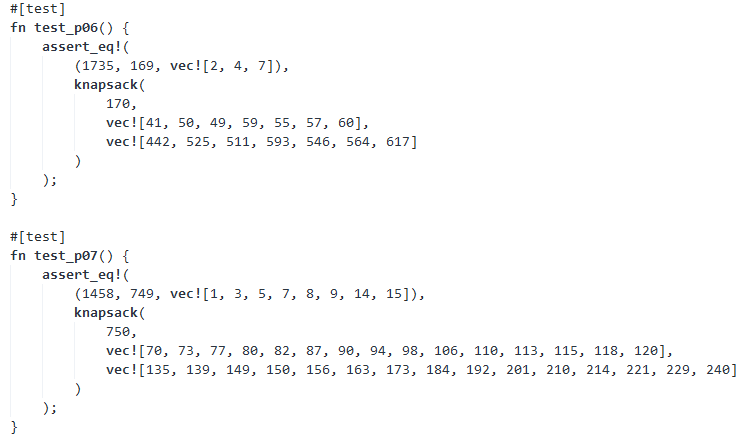
\includegraphics[scale=0.6]{content/images/impl_knapsack9.png}
  \caption{Второй набор тестов.}
  \label{fig:impl_knapsack9}
\end{figure}

Результатом выполнения программы является проверка всех тестов и вывод сообщения об успешном или провальном прохождении этих тестов. 

Полный кода листинг программы указан в приложении. (\hyperref[sec:appendix2]{Приложение Б})


\subsection{Задача о распределении инвестиций}

\indent Перед разработкой программной реализации решения задачи о замене оборудования было приведено аналитическое решение в среде MS Excel и там был автоматизирован процесс оптимизации в соответствие с математическими формулами.

Рассмотрим решение, которое было получено в среде MS Excel с помощью надстройки <<Поиск решения>>.

Имеется следующий набор исходных данных.
\begin{figure}[h]
  \centering 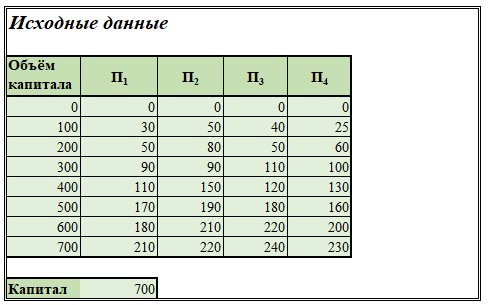
\includegraphics[scale=0.8]{content/images/impl_investing1.png}
  \caption{Исходные данные.}
  \label{fig:impl_investing1}
\end{figure}

Для решения данной задачи построим вспомогательную таблицу.
\begin{figure}[h]
  \centering 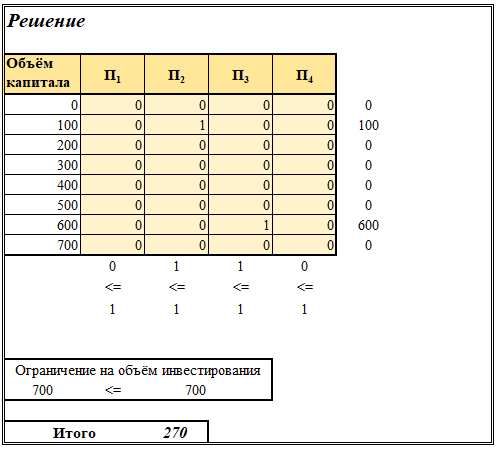
\includegraphics[scale=0.8]{content/images/impl_investing2.png}
  \caption{Таблица решения.}
  \label{fig:impl_investing2}
\end{figure}

Жёлтым цветом в таблице выделены ячейки, которые являются бинарными переменными в данной задаче и показывают будет ли вложение некоторого объёма капитала в данное предприятие. Ниже указано ограничение на то, что мы может только один раз проинвестировать в предприятие. Справа от таблицы с переменными указан столбец, который показывает объём капиталовложения в соответствующее предприятие. Снизу от таблицы указано ограничение на суммарное количество инвестиций, которое не должно превышать объёма капитала. Также под данным ограничением указано значение целевой функции (максимальная прибыль), которое находится как сумма произведения таблицы с переменными задачи и таблицы с исходными данными.

Исходя из этого мы можем применить <<Поиск решения>>.
\begin{figure}[h]
  \centering 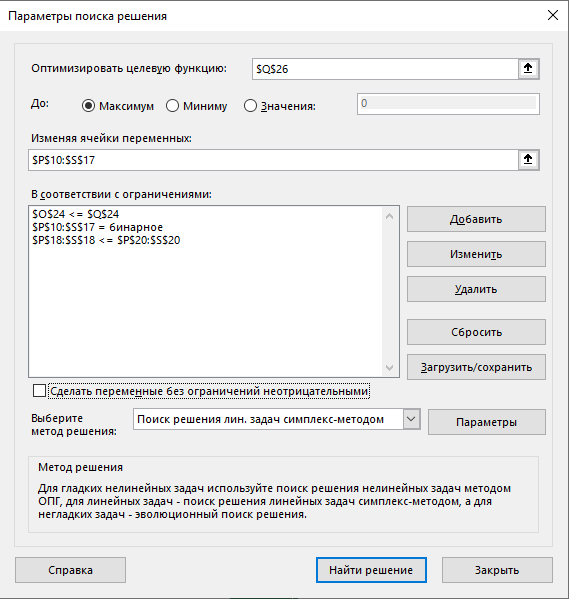
\includegraphics[scale=0.7]{content/images/impl_investing3.png}
  \caption{Окно <<Поиск решения>>.}
  \label{fig:impl_investing3}
\end{figure}

После этого можно увидеть получившееся решение и определить сколько стоит инвестировать в какое предприятие.
